\chapter{ВЫБОР ОПТИМАЛЬНОГО МЕТОДА ПОСТРОЕНИЯ СУРРОГАТНЫХ МОДЕЛЕЙ}\label{app:choosing-the-best-surrogate-model-method}

В рамках исследования методов построения суррогатных моделей
для многокритериальной оптимизации алгоритмов управления
электропневматическими приводами с дискретными распределителями
был применен метод морфологического анализа Фрица Цвикки. Данный
метод позволяет систематически рассмотреть все возможные решения
проблемы путем анализа всех комбинаций параметров, что особенно важно
при выборе оптимального подхода в сложных многопараметрических задачах.

Метод Цвикки включает в себя несколько этапов. На первом этапе
формулируется проблема и определяются ключевые параметры,
характеризующие возможные решения. В нашем случае, ключевыми
параметрами для оценки методов построения суррогатных моделей были выбраны:

A. Способность к аппроксимации нелинейных зависимостей
B. Масштабируемость
C. Вычислительная эффективность
D. Интерпретируемость результатов
E. Способность к обобщению
F. Адаптивность к типам данных
G. Оценка неопределенности

Для каждого параметра были определены возможные значения:
низкое, среднее и высокое (или эквивалентные им).
Это позволяет создать морфологическую матрицу,
которая представляет собой многомерное пространство возможных решений.

\begin{table}[h]
	\centering
	\caption{Морфологическая матрица методов построения суррогатных моделей}
	\begin{tabular}{lccc}
		\midrule
		Параметр                          & Значение 1 & Значение 2 & Значение 3 \\
		\midrule
		A. Способность к аппроксимации    & Низкая     & Средняя    & Высокая    \\
		нелинейных зависимостей           &            &            &            \\

		B. Масштабируемость               & Плохая     & Средняя    & Хорошая    \\
		C. Вычислительная эффективность   & Низкая     & Средняя    & Высокая    \\
		D. Интерпретируемость результатов & Низкая     & Средняя    & Высокая    \\
		E. Способность к обобщению        & Низкая     & Средняя    & Высокая    \\
		F. Адаптивность к типам данных    & Низкая     & Средняя    & Высокая    \\
		G. Оценка неопределенности        & Нет        & Частичная  & Полная     \\
		\midrule
	\end{tabular}
	\label{tab:morphological_matrix}
\end{table}

На следующем этапе анализа каждый рассматриваемый метод
построения суррогатных моделей был оценен по каждому параметру.
Оценка проводилась на основе теоретических свойств методов и опыта
их применения в схожих задачах. Результаты оценки представлены в следующей таблице:

\begin{table}[h]
	\centering
	\caption{Оценка методов по параметрам}
	\begin{tabular}{l|c|c|c|c|c|c|c}
		\midrule
		Метод                             & A & B & C & D & E & F & G \\
		\midrule
		Полиномиальная регрессия          & 1 & 1 & 3 & 3 & 1 & 1 & 1 \\
		\hline
		Радиальные базисные функции (RBF) & 2 & 2 & 2 & 2 & 2 & 2 & 1 \\
		\hline
		Кригинг (Гауссовы процессы)       & 2 & 1 & 1 & 1 & 3 & 2 & 3 \\
		\hline
		Метод опорных векторов (SVM)      & 2 & 3 & 2 & 1 & 3 & 2 & 1 \\
		\hline
		Нейронные сети                    & 3 & 3 & 2 & 1 & 3 & 3 & 2 \\
		\midrule
	\end{tabular}
	\label{tab:method_evaluation}
\end{table}

Здесь числовые значения соответствуют оценкам из
морфологической матрицы (1 -- низкая/плохая, 2 -- средняя, 3 -- высокая/хорошая).

Для наглядного представления результатов анализа на рисунке \ref{fig:morphological_analysis}
была приведена лепестковая диаграмма, отражающая оценки методов по каждому из
рассмотренных параметров.

\begin{figure}[ht]
	\centerfloat{
		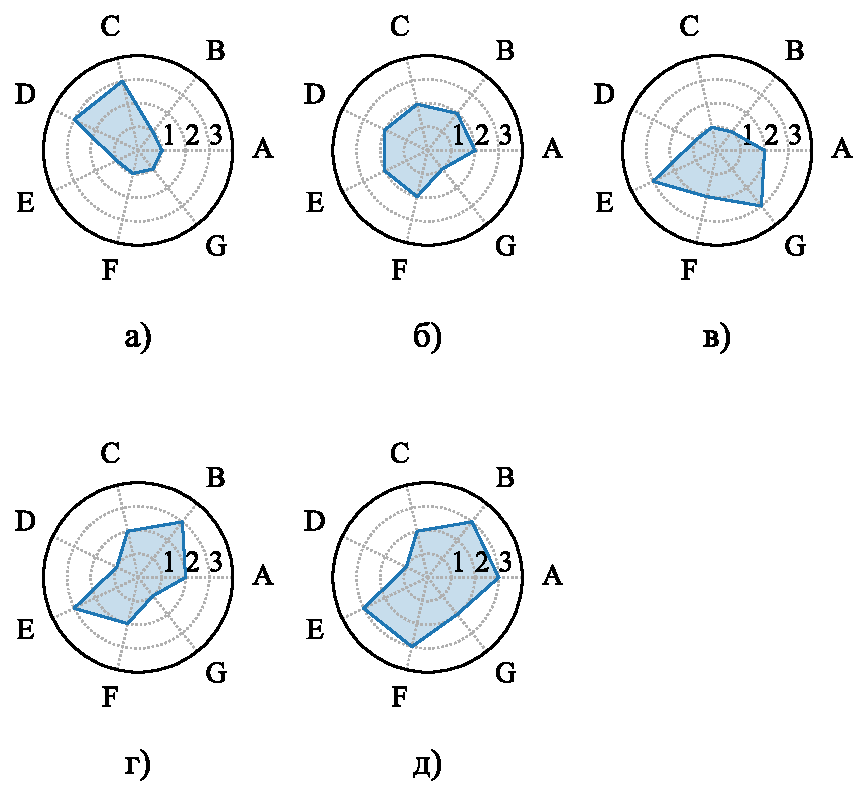
\includegraphics{part4/morphological_analyse.pdf}
	}
	\caption{Лепестковые диаграммы каждого варианта}\label{fig:morphological_analysis}
\end{figure}

Для выбора оптимального метода необходимо учитывать важность
каждого параметра в контексте нашей конкретной задачи.
Учитывая специфику многокритериальной оптимизации алгоритмов
управления электропневматическими приводами с дискретными
распределителями, были присвоены следующие веса параметрам:

\begin{itemize}
	\item A: 0.25 -- высокая важность из-за нелинейности системы;
	\item B: 0.20 -- важно для работы с множеством параметров;
	\item C: 0.15 -- важно для итеративного процесса оптимизации;
	\item D: 0.05 -- менее важно для данной задачи;
	\item E: 0.20 -- важно для работы с новыми комбинациями параметров;
	\item F: 0.10 -- важно для работы с различными типами параметров;
	\item G: 0.05 -- менее важно для данной задачи.
\end{itemize}

Используя эти веса, была вычислена взвешенная сумма для каждого метода. Рассмотрим пример расчета взвешенной суммы для метода нейронных сетей:

\begin{equation}
	\begin{split}
		S_{НС} = & 0.25 \cdot 3 + 0.20 \cdot 3 + 0.15 \cdot 2 + 0.05 \cdot 1 + \\
		+        & 0.20 \cdot 3 + 0.10 \cdot 3 + 0.05 \cdot 2 =                \\
		=        & 0.75 + 0.60 + 0.30 + 0.05 + 0.60 + 0.30 + 0.10 =            \\
		=        & 2.60
	\end{split}
\end{equation}
где $S_{НС}$ -- взвешенная сумма для нейронных сетей, а числовые значения
соответствуют оценкам из таблицы \ref{tab:method_evaluation}.

Аналогичным образом были рассчитаны взвешенные суммы для остальных методов.
Результаты представлены в таблице \ref{tab:weighted_scores}.

\begin{table}[h]
	\centering
	\caption{Взвешенные оценки методов}
	\begin{tabular}{lc}
		\midrule
		Метод                             & Взвешенная сумма \\
		\midrule
		Полиномиальная регрессия          & 1.60             \\
		Радиальные базисные функции (RBF) & 1.95             \\
		Кригинг (Гауссовы процессы)       & 1.90             \\
		Метод опорных векторов (SVM)      & 2.25             \\
		Нейронные сети                    & 2.60             \\
		\hline
	\end{tabular}
	\label{tab:weighted_scores}
\end{table}

Как видно из результатов, нейронные сети получили наивысшую взвешенную оценку
(2.60). Это объясняется тем, что они имеют высокие оценки по наиболее важным
критериям: способности к аппроксимации нелинейных зависимостей (вес 0.25),
масштабируемости (вес 0.20) и способности к обобщению (вес 0.20). Несмотря на
относительно низкую оценку по интерпретируемости результатов (1 с весом 0.05),
это не оказало значительного влияния на общий результат из-за низкого веса этого
критерия для нашей задачи.

На основе проведенного морфологического анализа с использованием метода
Цвикки, наиболее подходящим методом для построения суррогатной модели
в контексте многокритериальной оптимизации алгоритмов управления
электропневматическими приводами с дискретными распределителями
являются нейронные сети. Они получили наивысшую взвешенную оценку
благодаря своим сильным сторонам: высокой способности к аппроксимации
сложных нелинейных зависимостей, хорошей масштабируемости и работе с
высокоразмерными данными, высокой способности к обобщению и высокой
адаптивности к различным типам данных.

Несмотря на некоторые недостатки, такие как относительно низкая интерпретируемость
результатов и средняя вычислительная эффективность,
преимущества нейронных сетей в контексте данной задачи перевешивают
их недостатки. Для минимизации этих недостатков могут быть применены методы
регуляризации, техники визуализации и интерпретации нейронных сетей, а
также оптимизация архитектуры сети для повышения вычислительной эффективности.